%%%%%%%%%%%%%%%%%%%% author.tex %%%%%%%%%%%%%%%%%%%%%%%%%%%%%%%%%%%
%
% sample root file for your "contribution" to a contributed volume
%
% Use this file as a template for your own input.
%
%%%%%%%%%%%%%%%% Springer %%%%%%%%%%%%%%%%%%%%%%%%%%%%%%%%%%


% RECOMMENDED %%%%%%%%%%%%%%%%%%%%%%%%%%%%%%%%%%%%%%%%%%%%%%%%%%%
\documentclass[graybox]{svmult}

% choose options for [] as required from the list
% in the Reference Guide

\usepackage{type1cm}        % activate if the above 3 fonts are
                            % not available on your system
%
\usepackage{makeidx}         % allows index generation
\usepackage{graphicx}        % standard LaTeX graphics tool
                             % when including figure files
\usepackage{multicol}        % used for the two-column index
\usepackage[bottom]{footmisc}% places footnotes at page bottom


\usepackage{newtxtext}       % 
\usepackage{newtxmath}       % selects Times Roman as basic font

\usepackage{url}

%%Nirav added
\newenvironment{spmatrix}[1]
 {\def\mysubscript{#1}\mathop\bgroup\begin{pmatrix}}
 {\end{pmatrix}\egroup_{\textstyle\mathstrut\mysubscript}}
\DeclareMathOperator{\Tr}{Tr}
\DeclareMathOperator{\spn}{span}
%%Nirav added over

% see the list of further useful packages
% in the Reference Guide

\makeindex             % used for the subject index
                       % please use the style svind.ist with
                       % your makeindex program

%%%%%%%%%%%%%%%%%%%%%%%%%%%%%%%%%%%%%%%%%%%%%%%%%%%%%%%%%%%%%%%%%%%%%%%%%%%%%%%%%%%%%%%%%

\begin{document}

\title*{Reduced order modeling of geometrically parametrized discontinuous Galerkin formulation for the Stokes equation}
% Use \titlerunning{Short Title} for an abbreviated version of
% your contribution title if the original one is too long
\author{Nirav Vasant Shah, Martin Hess and Gianluigi Rozza}
% Use \authorrunning{Short Title} for an abbreviated version of
% your contribution title if the original one is too long
\institute{Nirav Vasant Shah \at Scuola Internazionale Superiore di Studi Avanzati - via Bonomea, 265 - 34136 Trieste ITALY, \email{snirav@sissa.it}
\and Martin Hess \at Scuola Internazionale Superiore di Studi Avanzati - via Bonomea, 265 - 34136 Trieste ITALY \email{martin.hess@sissa.it}}
%
% Use the package "url.sty" to avoid
% problems with special characters
% used in your e-mail or web address
%
\maketitle

\abstract*{Each chapter should be preceded by an abstract (no more than 200 words) that summarizes the content. The abstract will appear \textit{online} at \url{www.SpringerLink.com} and be available with unrestricted access. This allows unregistered users to read the abstract as a teaser for the complete chapter.
Please use the 'starred' version of the \texttt{abstract} command for typesetting the text of the online abstracts (cf. source file of this chapter template \texttt{abstract}) and include them with the source files of your manuscript. Use the plain \texttt{abstract} command if the abstract is also to appear in the printed version of the book.}

\abstract{The present work focuses on geometrical parametrization and reduced order modeling of Stokes flow. The importance of Stokes flow, advantages of discontinuous Galerkin method are introduced first. We also discuss the concept of geometric parametrization and its application along with importance of reduced order model technique.  The full order model is based on discontinuous Galerkin method interior penalty formulation. The concepts of broken Sobolev spaces, relevant norms, jump and mean operator are introduced. The weak formulation is derived based in suitable space to obtain the full order model. We then introduce the concept of geometric parametrization. The operators are transformed from fixed domain to parameter dependent domain by exploring affine parameter dependence which results in efficient assembly of system matrix. Thereafter, proper orthogonal decomposition is applied to obtain basis for function space for reduced order model. By using Galerkin projection the linear system to be solved is projected onto reduced space. During the process, offline-online decomposition is used to separate computation of expensive parameter independent part and fast parameter independent part. Finally the technique is applied to test problem. The numerical outcomes presented include the experimental error analysis, eigenvalue computation and measurement of online simulation time. \cite{psysoc-journal}}

\section{Introduction}
\label{introduction}

The subject of mathematical applications in fluid mechanics starts with one of the variants of the Navier-Stokes equations, such as the Stokes equation. Almost all processes of fluid mechanics require considerations related to the Navier-Stokes equations. Navier-Stokes equation is non-linear, characterizing flow fluctuations. However, in case of laminar flow, i.e. when fluctuations are negligible, this linearized form of the Navier-Stokes equation is the Stokes equation.

Discontinuous Galerkin method (DGM) has found traction as numerical method for elliptic problems \textbf{pereire reference} as well as hyperbolic problems \textbf{Book on compressible flow reference}. This is due to its several advantages over Finite Element Method (FEM) and Finite Volume Method (FVM). In fact, DG method is considered as combination of FEM and FVM. DGM uses polynomial approximation of suitable degree providing higher accuracy as well as allows discontinuity at the interface, by the concept of numerical flux, allowing greater flexibility. This fact makes DGM naturally attractive to problems such as shock capturing due to presence of steep gradients or discontinuities. Additionally, since the Dirichlet conditions are applied as boundary penalty, it avoids necessity to work with subspace of FEM. Several variants of DGM exist based on computational advantages such as sparsity pattern or extension of computational stencil, complexity of numerical implementation etc.

Geometric parametrization has emerged as important application of Parametric Partial Differential Equations (PPDEs) and as alternative to shape optimization. The concept of geometric parametrization allows to transfer operator evaluated on one domain to another domain efficiently. For linear equations, this means exploiting affine parameter dependence as will be shown in later section. Model Order Reduction (MOR) on the other hand allows reducing the size of the system to be solved and working with the smaller system containing only dominant components and discarding the non-dominant components. It is pertinent to mention that identifying "dominant" components is critical to the success of model order reduction strategy. Optimization of engineering components using geometric parametrization combined with MOR for PPDEs has given quite useful results in the fields such as mechanical, naval and aeronautic designs. Also, the  faster computations obtained by MOR has helped in many query context, real time computation and quick transfer of computational results to industrial problems.

In the present work, we first introduce Discontinuous Galerkin Interior Penalty Method (DG-IPM). We subsequently introduce notion of parametrization characterizing geometry of the domain under consideration, exploit affine parameter dependence and its application in the context of offline-online decomposition. We then apply Proper Orthogonal Decomposition (POD) for constructing reduced basis space and apply Galerkin projection to project the system of equations on the space constructed by POD. Finally we present a test problem to demonstrate the introduced method and present numerical result.
 
\section{Discontinuous Galerkin formulation}
\label{DG_formulation}

Let $\Omega \subset \mathbb{R}^d$ be open bounded domain. The boundary of $\Omega$, $\partial \Omega$ is divided into Neumann boundary $\Gamma_N$ and Dirichlet boundary $\Gamma_D$ i.e. $\partial \Omega = \Gamma_N \cup \Gamma_D$. The domain $\Omega$ is divide into $N_{su}$ number of mutually non overlapping subdomains such that, $\Omega = \bigcup\limits_{i=1}^{N_{su}} \Omega_i \ , \ \Omega_i \cap \Omega_j = \emptyset \ , \ \text{for } i \neq j$. Each subdomain is divided into $nel$ number of triangular elements $\tau_k$ such that $\Omega = \bigcup\limits_{k=1}^{nel} \tau_k$. The triangulation $\mathcal{T}$ is the set of all triangular elements i.e. $\mathcal{T} = \lbrace \tau_k \rbrace_{k=1}^{nel}$. The internal boundary $\Gamma = \lbrace \partial \tau_k \rbrace_{k=1}^{nel} \backslash \partial \Omega$. We represent $\overrightarrow{n}$ as the outward pointing normal to an edge of element.

The Stokes's equation in strong form can be stated as,
\begin{gather}
-\nu \Delta \overrightarrow{u} + \nabla p = \overrightarrow{f} \ , \ \text{in } \Omega \ , \\
\nabla \cdot \overrightarrow{u} = 0 \ , \\
\overrightarrow{u} = \overrightarrow{u}_D \ , \ \text{on } \Gamma_D \ , \\
-p \overrightarrow{n} + \nu \overrightarrow{n} \cdot \nabla \overrightarrow{u} = \overrightarrow{t} \ , \ \text{on } \Gamma_N \ .
\end{gather}

The vector variable velocity $\overrightarrow{u}$ and scalar pressure $p$ are the unknowns. $\nu$ is the material property known as kinematic viscosity. Vector $\overrightarrow{f}$ is external force term or source term. $\overrightarrow{u}_D$ is the Dirichlet velocity and $\overrightarrow{t}$ is the Neumann value.

Before introducing weak form let us introduce broken Sobolev spaces for variables. 
The space for velocity is 
\begin{equation} \label{velocity_test}
\mathbb{V} = \lbrace \overrightarrow{\phi} \in (L^2(\mathcal{T}))^d| \quad \overrightarrow{\phi} \in (P^D(\tau_k))^d \quad \forall \quad {\tau_k} \in \mathcal{T} \rbrace \ .
\end{equation}
The space for pressure is 
\begin{equation} \label{pressure_test}
\mathbb{Q} = \lbrace \psi \in (L^2(\mathcal{T}))| \quad \psi \in (P^{D-1}(\tau_k)) \quad \forall \quad {\tau_k} \in \mathcal{T} \rbrace \ .
\end{equation}
Here, $P^D(\tau_k)$ denotes space of polynomials of degree at most $D$ over $\tau_k$.

In order to approximate the numerical flux we need the concept of Jump and Average operator. 
1.  For scalar quantity $p$ the jump operator is defined as,
\begin{equation}
\begin{split}
[p\overrightarrow{n}] = p^+ \overrightarrow{n}^+ + p^- \overrightarrow{n}^- \quad \textrm{on} \quad \Gamma \textrm{,}\\
[p\overrightarrow{n}] = p \overrightarrow{n} \quad \textrm{on} \quad \Gamma_D \textrm{.}
\end{split}
\end{equation}

2. For vector quantity $\overrightarrow{u}$ the jump operator is defined as,
\begin{equation}
\begin{split}
[\overrightarrow{n} \cdot \overrightarrow{u}] = \overrightarrow{n}^+ \cdot \overrightarrow{u}^+ + \overrightarrow{n}^- \cdot \overrightarrow{u}^- \quad \textrm{on} \quad \Gamma \textrm{,}\\
[\overrightarrow{n} \cdot \overrightarrow{u}] = \overrightarrow{n} \cdot \overrightarrow{u} \quad \textrm{on} \quad \Gamma_D \textrm{.}\\
\end{split}
\end{equation}

3. The average operator is defined as,
\begin{equation}\label{average operator}
\left\lbrace \overrightarrow{u} \right\rbrace = \frac{\overrightarrow{u}^+ + \overrightarrow{u}^-}{2} \textrm{.}
\end{equation} 

The weak form of Stokes equation is as follow,

\begin{equation}\label{stokes_weak_ch3}
\begin{split}
a_{IP}(\overrightarrow{u},\overrightarrow{\phi}) + b(\overrightarrow{\phi},p) + (\lbrace p \rbrace,[\overrightarrow{n} \cdot \overrightarrow{\phi}])_{\Gamma \cup \Gamma_D} = l_{IP}(\overrightarrow{\phi}) \ .
\end{split}
\end{equation}

\begin{equation}\label{a_IP}
\begin{split}
a_{IP}(\overrightarrow{u},\overrightarrow{\phi}) = (\nabla \overrightarrow{u}, \nabla \overrightarrow{\phi}) + C_{11} ([\overrightarrow{u}],[\overrightarrow{\phi}])_{\Gamma \cup \Gamma_D} \\
- \nu ({\nabla \overrightarrow{u}},[\overrightarrow{n} \otimes \overrightarrow{\phi}])_{\Gamma \cup \Gamma_D} - \nu ([\overrightarrow{n} \otimes \overrightarrow{u}],{\nabla \overrightarrow{\phi}})_{\Gamma \cup \Gamma_D} \textrm{.}
\end{split}
\end{equation}

The penalty paramter $C_{11}>0$ is an empirical constant to be kept large enough to maintain coercivity of bilinear form.

\begin{equation}\label{b}
b(\phi,\psi) = -\int_{\mathcal{T}} \psi \nabla \cdot \overrightarrow{\phi} \ ,
\end{equation}

\begin{equation}\label{l_IP}
\begin{split}
l_{IP}(\overrightarrow{\phi}) = (\overrightarrow{f},\overrightarrow{\phi}) + (\overrightarrow{t},\overrightarrow{\phi})_{\Gamma_N} + C_{11} (\overrightarrow{u}_D,\overrightarrow{\phi})_{\Gamma_D} - (\overrightarrow{n} \otimes \overrightarrow{u}_D, \nu \nabla \overrightarrow{\phi})_{\Gamma_D} \ .
\end{split}
\end{equation}

Discrete form of equations can be written in Matrix form as, 

\begin{equation} \label{Stokes_matrix_ch3}
\begin{spmatrix}{\textrm{Stiffness matrix}}
    A & B \\
    B^T & 0
\end{spmatrix}
\begin{spmatrix}{\textrm{Solution vector}}
    U \\
    P
\end{spmatrix}
=
\begin{spmatrix}{\textrm{Right hand side (Known)}}
    F_1  \\
    F_2
\end{spmatrix}
\textrm{.}
\end{equation}

Here, 
\begin{equation} \label{matrix A}
\begin{split}
A_{ij} = \sum_{k=1}^d (\frac{\partial \phi_i}{\partial x_k} , \frac{\partial \phi_j}{\partial x_k}) + \sum_{k=1}^d C_{11} ([\phi_i n_k] , [\phi_j n_k])_{\Gamma \cup \Gamma_D} \\ - \sum_{k=1}^d \nu ([\phi_i n_k] , \lbrace \frac{\partial \phi_j}{\partial x_k} \rbrace)_{\Gamma \cup \Gamma_D} - \sum_{k=1}^d \nu (\lbrace \frac{\partial \phi_i}{\partial x_k} \rbrace , [\phi_j n_k])_{\Gamma \cup \Gamma_D} \ .
\end{split}
\end{equation}

\begin{equation} \label{matrix B}
B_{ij} = - \int_{\mathcal{T}} \frac{\partial \phi_i}{\partial x_i} \psi_j +
(\lbrace \psi_j \rbrace , [n \cdot \phi_i])_{\Gamma \cup \Gamma_D} \ .
\end{equation}



\begin{enumerate}
\item{Livelihood and survival mobility are oftentimes coutcomes of uneven socioeconomic development.}
\begin{enumerate}
\item{Livelihood and survival mobility are oftentimes coutcomes of uneven socioeconomic development.}
\item{Livelihood and survival mobility are oftentimes coutcomes of uneven socioeconomic development.}
\end{enumerate}
\item{Livelihood and survival mobility are oftentimes coutcomes of uneven socioeconomic development.}
\end{enumerate}


\subparagraph{Subparagraph Heading} In order to avoid simply listing headings of different levels we recommend to let every heading be followed by at least a short passage of text. Use the \LaTeX\ automatism for all your cross-references and citations as has already been described in Sect.~\ref{sec:2}, see also Fig.~\ref{fig:2}.

For unnumbered list we recommend to use the \verb|itemize| environment -- it will automatically be rendered in line with the preferred layout.

\begin{itemize}
\item{Livelihood and survival mobility are oftentimes coutcomes of uneven socioeconomic development, cf. Table~\ref{tab:1}.}
\begin{itemize}
\item{Livelihood and survival mobility are oftentimes coutcomes of uneven socioeconomic development.}
\item{Livelihood and survival mobility are oftentimes coutcomes of uneven socioeconomic development.}
\end{itemize}
\item{Livelihood and survival mobility are oftentimes coutcomes of uneven socioeconomic development.}
\end{itemize}

\begin{figure}[t]
\sidecaption[t]
% Use the relevant command for your figure-insertion program
% to insert the figure file.
% For example, with the option graphics use
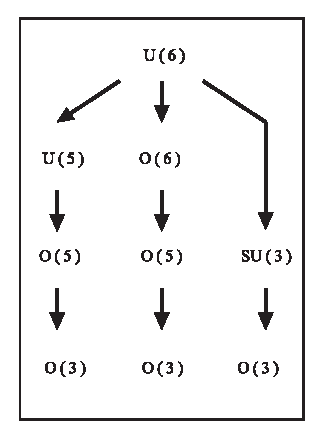
\includegraphics[scale=.65]{figure}
%
% If no graphics program available, insert a blank space i.e. use
%\picplace{5cm}{2cm} % Give the correct figure height and width in cm
%
%\caption{Please write your figure caption here}
\caption{If the width of the figure is less than 7.8 cm use the \texttt{sidecapion} command to flush the caption on the left side of the page. If the figure is positioned at the top of the page, align the sidecaption with the top of the figure -- to achieve this you simply need to use the optional argument \texttt{[t]} with the \texttt{sidecaption} command}
\label{fig:2}       % Give a unique label
\end{figure}

\runinhead{Run-in Heading Boldface Version} Use the \LaTeX\ automatism for all your cross-references and citations as has already been described in Sect.~\ref{sec:2}.

\subruninhead{Run-in Heading Boldface and Italic Version} Use the \LaTeX\ automatism for all your cross-refer\-ences and citations as has already been described in Sect.~\ref{sec:2}\index{paragraph}.

\subsubruninhead{Run-in Heading Displayed Version} Use the \LaTeX\ automatism for all your cross-refer\-ences and citations as has already been described in Sect.~\ref{sec:2}\index{paragraph}.
% Use the \index{} command to code your index words
%
% For tables use
%
\begin{table}[!t]
\caption{Please write your table caption here}
\label{tab:1}       % Give a unique label
%
% Follow this input for your own table layout
%
\begin{tabular}{p{2cm}p{2.4cm}p{2cm}p{4.9cm}}
\hline\noalign{\smallskip}
Classes & Subclass & Length & Action Mechanism  \\
\noalign{\smallskip}\svhline\noalign{\smallskip}
Translation & mRNA$^a$  & 22 (19--25) & Translation repression, mRNA cleavage\\
Translation & mRNA cleavage & 21 & mRNA cleavage\\
Translation & mRNA  & 21--22 & mRNA cleavage\\
Translation & mRNA  & 24--26 & Histone and DNA Modification\\
\noalign{\smallskip}\hline\noalign{\smallskip}
\end{tabular}
$^a$ Table foot note (with superscript)
\end{table}
%
\section{Section Heading}
\label{sec:3}
% Always give a unique label
% and use \ref{<label>} for cross-references
% and \cite{<label>} for bibliographic references
% use \sectionmark{}
% to alter or adjust the section heading in the running head
Instead of simply listing headings of different levels we recommend to let every heading be followed by at least a short passage of text.  Further on please use the \LaTeX\ automatism for all your cross-references and citations as has already been described in Sect.~\ref{sec:2}.

Please note that the first line of text that follows a heading is not indented, whereas the first lines of all subsequent paragraphs are.

If you want to list definitions or the like we recommend to use the enhanced \verb|description| environment -- it will automatically rendered in line with the preferred layout.

\begin{description}[Type 1]
\item[Type 1]{That addresses central themes pertainng to migration, health, and disease. In Sect.~\ref{sec:1}, Wilson discusses the role of human migration in infectious disease distributions and patterns.}
\item[Type 2]{That addresses central themes pertainng to migration, health, and disease. In Sect.~\ref{subsec:2}, Wilson discusses the role of human migration in infectious disease distributions and patterns.}
\end{description}

\subsection{Subsection Heading} %
In order to avoid simply listing headings of different levels we recommend to let every heading be followed by at least a short passage of text. Use the \LaTeX\ automatism for all your cross-references and citations citations as has already been described in Sect.~\ref{sec:2}.

Please note that the first line of text that follows a heading is not indented, whereas the first lines of all subsequent paragraphs are.

\begin{svgraybox}
If you want to emphasize complete paragraphs of texts we recommend to use the newly defined class option \verb|graybox| and the newly defined environment \verb|svgraybox|. This will produce a 15 percent screened box 'behind' your text.

If you want to emphasize complete paragraphs of texts we recommend to use the newly defined class option and environment \verb|svgraybox|. This will produce a 15 percent screened box 'behind' your text.
\end{svgraybox}


\subsubsection{Subsubsection Heading}
Instead of simply listing headings of different levels we recommend to let every heading be followed by at least a short passage of text.  Further on please use the \LaTeX\ automatism for all your cross-references and citations as has already been described in Sect.~\ref{sec:2}.

Please note that the first line of text that follows a heading is not indented, whereas the first lines of all subsequent paragraphs are.

\begin{theorem}
Theorem text goes here.
\end{theorem}
%
% or
%
\begin{definition}
Definition text goes here.
\end{definition}

\begin{proof}
%\smartqed
Proof text goes here.
%\qed
\end{proof}

\paragraph{Paragraph Heading} %
Instead of simply listing headings of different levels we recommend to let every heading be followed by at least a short passage of text.  Further on please use the \LaTeX\ automatism for all your cross-references and citations as has already been described in Sect.~\ref{sec:2}.

Note that the first line of text that follows a heading is not indented, whereas the first lines of all subsequent paragraphs are.
%
% For built-in environments use
%
\begin{theorem}
Theorem text goes here.
\end{theorem}
%
\begin{definition}
Definition text goes here.
\end{definition}
%
\begin{proof}
%\smartqed
Proof text goes here.
%\qed
\end{proof}
%
\begin{trailer}{Trailer Head}
If you want to emphasize complete paragraphs of texts in an \verb|Trailer Head| we recommend to
use  \begin{verbatim}\begin{trailer}{Trailer Head}
...
\end{trailer}\end{verbatim}
\end{trailer}
%
\begin{question}{Questions}
If you want to emphasize complete paragraphs of texts in an \verb|Questions| we recommend to
use  \begin{verbatim}\begin{question}{Questions}
...
\end{question}\end{verbatim}
\end{question}
\eject%
\begin{important}{Important}
If you want to emphasize complete paragraphs of texts in an \verb|Important| we recommend to
use  \begin{verbatim}\begin{important}{Important}
...
\end{important}\end{verbatim}
\end{important}
%
\begin{warning}{Attention}
If you want to emphasize complete paragraphs of texts in an \verb|Attention| we recommend to
use  \begin{verbatim}\begin{warning}{Attention}
...
\end{warning}\end{verbatim}
\end{warning}

\begin{programcode}{Program Code}
If you want to emphasize complete paragraphs of texts in an \verb|Program Code| we recommend to
use

\verb|\begin{programcode}{Program Code}|

\verb|\begin{verbatim}...\end{verbatim}|

\verb|\end{programcode}|

\end{programcode}
%
\begin{tips}{Tips}
If you want to emphasize complete paragraphs of texts in an \verb|Tips| we recommend to
use  \begin{verbatim}\begin{tips}{Tips}
...
\end{tips}\end{verbatim}
\end{tips}
\eject
%
\begin{overview}{Overview}
If you want to emphasize complete paragraphs of texts in an \verb|Overview| we recommend to
use  \begin{verbatim}\begin{overview}{Overview}
...
\end{overview}\end{verbatim}
\end{overview}
\begin{backgroundinformation}{Background Information}
If you want to emphasize complete paragraphs of texts in an \verb|Background|
\verb|Information| we recommend to
use

\verb|\begin{backgroundinformation}{Background Information}|

\verb|...|

\verb|\end{backgroundinformation}|
\end{backgroundinformation}
\begin{legaltext}{Legal Text}
If you want to emphasize complete paragraphs of texts in an \verb|Legal Text| we recommend to
use  \begin{verbatim}\begin{legaltext}{Legal Text}
...
\end{legaltext}\end{verbatim}
\end{legaltext}
%
\begin{acknowledgement}
If you want to include acknowledgments of assistance and the like at the end of an individual chapter please use the \verb|acknowledgement| environment -- it will automatically be rendered in line with the preferred layout.
\end{acknowledgement}
%
\section*{Appendix}
\addcontentsline{toc}{section}{Appendix}
%
%
When placed at the end of a chapter or contribution (as opposed to at the end of the book), the numbering of tables, figures, and equations in the appendix section continues on from that in the main text. Hence please \textit{do not} use the \verb|appendix| command when writing an appendix at the end of your chapter or contribution. If there is only one the appendix is designated ``Appendix'', or ``Appendix 1'', or ``Appendix 2'', etc. if there is more than one.

\begin{equation}
a \times b = c
\end{equation}

\bibliographystyle{spbasic.bst}
\bibliography{references.tex}
%%%%%%%%%%%%%%%%%%%%%%%% referenc.tex %%%%%%%%%%%%%%%%%%%%%%%%%%%%%%
% sample references
% %
% Use this file as a template for your own input.
%
%%%%%%%%%%%%%%%%%%%%%%%% Springer-Verlag %%%%%%%%%%%%%%%%%%%%%%%%%%
%
% BibTeX users please use
% \bibliographystyle{}
% \bibliography{}
%
\biblstarthook{References may be \textit{cited} in the text either by number (preferred) or by author/year.\footnote{Make sure that all references from the list are cited in the text. Those not cited should be moved to a separate \textit{Further Reading} section or chapter.} If the citatiion in the text is numbered, the reference list should be arranged in ascending order. If the citation in the text is author/year, the reference list should be \textit{sorted} alphabetically and if there are several works by the same author, the following order should be used:
\begin{enumerate}
\item all works by the author alone, ordered chronologically by year of publication
\item all works by the author with a coauthor, ordered alphabetically by coauthor
\item all works by the author with several coauthors, ordered chronologically by year of publication.
\end{enumerate}
The \textit{styling} of references\footnote{Always use the standard abbreviation of a journal's name according to the ISSN \textit{List of Title Word Abbreviations}, see \url{http://www.issn.org/en/node/344}} depends on the subject of your book:
\begin{itemize}
\item The \textit{two} recommended styles for references in books on \textit{mathematical, physical, statistical and computer sciences} are depicted in ~\cite{science-contrib, science-online, science-mono, science-journal, science-DOI} and ~\cite{phys-online, phys-mono, phys-journal, phys-DOI, phys-contrib}.
\item Examples of the most commonly used reference style in books on \textit{Psychology, Social Sciences} are~\cite{psysoc-mono, psysoc-online,psysoc-journal, psysoc-contrib, psysoc-DOI}.
\item Examples for references in books on \textit{Humanities, Linguistics, Philosophy} are~\cite{humlinphil-journal, humlinphil-contrib, humlinphil-mono, humlinphil-online, humlinphil-DOI}.
\item Examples of the basic Springer Nature style used in publications on a wide range of subjects such as \textit{Computer Science, Economics, Engineering, Geosciences, Life Sciences, Medicine, Biomedicine} are ~\cite{basic-contrib, basic-online, basic-journal, basic-DOI, basic-mono}. 
\end{itemize}
}

\begin{thebibliography}{99.}%
% and use \bibitem to create references.
%
% Use the following syntax and markup for your references if 
% the subject of your book is from the field 
% "Mathematics, Physics, Statistics, Computer Science"
%
% Contribution 
\bibitem{science-contrib} Broy, M.: Software engineering --- from auxiliary to key technologies. In: Broy, M., Dener, E. (eds.) Software Pioneers, pp. 10-13. Springer, Heidelberg (2002)
%
% Online Document
\bibitem{science-online} Dod, J.: Effective substances. In: The Dictionary of Substances and Their Effects. Royal Society of Chemistry (1999) Available via DIALOG. \\
\url{http://www.rsc.org/dose/title of subordinate document. Cited 15 Jan 1999}
%
% Monograph
\bibitem{science-mono} Geddes, K.O., Czapor, S.R., Labahn, G.: Algorithms for Computer Algebra. Kluwer, Boston (1992) 
%
% Journal article
\bibitem{science-journal} Hamburger, C.: Quasimonotonicity, regularity and duality for nonlinear systems of partial differential equations. Ann. Mat. Pura. Appl. \textbf{169}, 321--354 (1995)
%
% Journal article by DOI
\bibitem{science-DOI} Slifka, M.K., Whitton, J.L.: Clinical implications of dysregulated cytokine production. J. Mol. Med. (2000) doi: 10.1007/s001090000086 
%
\bigskip

% Use the following (APS) syntax and markup for your references if 
% the subject of your book is from the field 
% "Mathematics, Physics, Statistics, Computer Science"
%
% Online Document
\bibitem{phys-online} J. Dod, in \textit{The Dictionary of Substances and Their Effects}, Royal Society of Chemistry. (Available via DIALOG, 1999), 
\url{http://www.rsc.org/dose/title of subordinate document. Cited 15 Jan 1999}
%
% Monograph
\bibitem{phys-mono} H. Ibach, H. L\"uth, \textit{Solid-State Physics}, 2nd edn. (Springer, New York, 1996), pp. 45-56 
%
% Journal article
\bibitem{phys-journal} S. Preuss, A. Demchuk Jr., M. Stuke, Appl. Phys. A \textbf{61}
%
% Journal article by DOI
\bibitem{phys-DOI} M.K. Slifka, J.L. Whitton, J. Mol. Med., doi: 10.1007/s001090000086
%
% Contribution 
\bibitem{phys-contrib} S.E. Smith, in \textit{Neuromuscular Junction}, ed. by E. Zaimis. Handbook of Experimental Pharmacology, vol 42 (Springer, Heidelberg, 1976), p. 593
%
\bigskip
%
% Use the following syntax and markup for your references if 
% the subject of your book is from the field 
% "Psychology, Social Sciences"
%
%
% Monograph
\bibitem{psysoc-mono} Calfee, R.~C., \& Valencia, R.~R. (1991). \textit{APA guide to preparing manuscripts for journal publication.} Washington, DC: American Psychological Association.
%
% Online Document
\bibitem{psysoc-online} Dod, J. (1999). Effective substances. In: The dictionary of substances and their effects. Royal Society of Chemistry. Available via DIALOG. \\
\url{http://www.rsc.org/dose/Effective substances.} Cited 15 Jan 1999.
%
% Journal article
\bibitem{psysoc-journal} Harris, M., Karper, E., Stacks, G., Hoffman, D., DeNiro, R., Cruz, P., et al. (2001). Writing labs and the Hollywood connection. \textit{J Film} Writing, 44(3), 213--245.
%
% Contribution 
\bibitem{psysoc-contrib} O'Neil, J.~M., \& Egan, J. (1992). Men's and women's gender role journeys: Metaphor for healing, transition, and transformation. In B.~R. Wainrig (Ed.), \textit{Gender issues across the life cycle} (pp. 107--123). New York: Springer.
%
% Journal article by DOI
\bibitem{psysoc-DOI}Kreger, M., Brindis, C.D., Manuel, D.M., Sassoubre, L. (2007). Lessons learned in systems change initiatives: benchmarks and indicators. \textit{American Journal of Community Psychology}, doi: 10.1007/s10464-007-9108-14.
%
%
% Use the following syntax and markup for your references if 
% the subject of your book is from the field 
% "Humanities, Linguistics, Philosophy"
%
\bigskip
%
% Journal article
\bibitem{humlinphil-journal} Alber John, Daniel C. O'Connell, and Sabine Kowal. 2002. Personal perspective in TV interviews. \textit{Pragmatics} 12:257--271
%
% Contribution 
\bibitem{humlinphil-contrib} Cameron, Deborah. 1997. Theoretical debates in feminist linguistics: Questions of sex and gender. In \textit{Gender and discourse}, ed. Ruth Wodak, 99--119. London: Sage Publications.
%
% Monograph
\bibitem{humlinphil-mono} Cameron, Deborah. 1985. \textit{Feminism and linguistic theory.} New York: St. Martin's Press.
%
% Online Document
\bibitem{humlinphil-online} Dod, Jake. 1999. Effective substances. In: The dictionary of substances and their effects. Royal Society of Chemistry. Available via DIALOG. \\
http://www.rsc.org/dose/title of subordinate document. Cited 15 Jan 1999
%
% Journal article by DOI
\bibitem{humlinphil-DOI} Suleiman, Camelia, Daniel C. O'Connell, and Sabine Kowal. 2002. `If you and I, if we, in this later day, lose that sacred fire...': Perspective in political interviews. \textit{Journal of Psycholinguistic Research}. doi: 10.1023/A:1015592129296.
%
%
%
\bigskip
%
%
% Use the following syntax and markup for your references if 
% the subject of your book is from the field 
% "Computer Science, Economics, Engineering, Geosciences, Life Sciences"
%
%
% Contribution 
\bibitem{basic-contrib} Brown B, Aaron M (2001) The politics of nature. In: Smith J (ed) The rise of modern genomics, 3rd edn. Wiley, New York 
%
% Online Document
\bibitem{basic-online} Dod J (1999) Effective Substances. In: The dictionary of substances and their effects. Royal Society of Chemistry. Available via DIALOG. \\
\url{http://www.rsc.org/dose/title of subordinate document. Cited 15 Jan 1999}
%
% Journal article by DOI
\bibitem{basic-DOI} Slifka MK, Whitton JL (2000) Clinical implications of dysregulated cytokine production. J Mol Med, doi: 10.1007/s001090000086
%
% Journal article
\bibitem{basic-journal} Smith J, Jones M Jr, Houghton L et al (1999) Future of health insurance. N Engl J Med 965:325--329
%
% Monograph
\bibitem{basic-mono} South J, Blass B (2001) The future of modern genomics. Blackwell, London 
%
\end{thebibliography}

\end{document}
